\documentclass[10pt,twocolumn]{article}

% use the oxycomps style file
\usepackage{oxycomps}
% usage: \fixme[comments describing issue]{text to be fixed}
% define \fixme as not doing anything special
\newcommand{\fixme}[2][]{#2}
% overwrite it so it shows up as red
\renewcommand{\fixme}[2][]{\textcolor{red}{#2}}
% overwrite it again so related text shows as footnotes
%\renewcommand{\fixme}[2][]{\textcolor{red}{#2\footnote{#1}}}

% read references.bib for the bibtex data
\bibliography{references}

% include metadata in the generated pdf file
\pdfinfo{
/Title (Preliminary Education of Traffic Engineering Using Sandboxes)
/Author (Matthew Perez)
}

% set the title and author information
\title{Preliminary Education of Traffic Engineering Using Sandboxes}
\author{Matthew Perez}
\affiliation{Occidental College}
\email{mperez2@oxy.edu}

\begin{document}

\maketitle

\section{Introduction and Problem Context}
\label{Introduction and Problem Context}

My Comprehensive project is a traffic simulator where the user able to create simple road networks with intersections, homes and offices, and individual cars. When I first started looking into urban planning and traffic engineering as a hobby, I often found much in both media, literature, and real life examples. I took a lot from my own personal research of traffic but was never really able to visualize it and create my own meaning from it, I was only able to attribute information I learned to real life examples. For example seeing how traffic flowed through a light signalled intersection versus a roundabout. 

With this issue my project sought to create a simulator designed around traffic management for beginners, catering to those with an interest in traffic but not knowing all details and metrics that go into traffic. As I, personally, was unable to find traffic simulators that were both easy to use for a new user and a simulator that solely focused on traffic. 

Although this project only scratched the surface of traffic simulation the amount of work required for the project was quite immense. With simulators many small pieces need to work together simultaneously and in many different situations in order to complete even simple tasks. An example of small pieces needing cooperation in my project, is cars working with roads and other cars, as throughout my work cars would repeatedly cause trouble with one another, such as clipping, stopping forever, or piling on top of one another, all of which caused by separate bugs in the simulation. Even now there may be bugs due to differing situations users can put cars into. 
\section{Technical Background}

Throughout this paper I will be using terms commonly spoken in the Unity game engine, along with more specialized computer science terms.

With these computer science terms the most prominent within the project is A-Star, a path finding algorithm used near always when implementing mapping and traversal. It is widely used for its cost effective finding of the cheapest path defined by the programmer, and in this case it is used to get a car from point A to point B. 

Unity also has some key terms used throughout the paper. Because unity is a game engine it is host to many unique functions relating to rendering, game frames, and spawning different objects. One of the most commonly used functions in my project is a Coroutine, which allows for methods to be run throughout multiple frames instead of all at once \cite{UnityManual}. Coroutines are especially useful for iterators or loops that can run for a large amount of time. A star is a good example as instead of running all at once and possible pausing the game until the path is complete, it will instead execute through multiple frames, meaning the simulator will not lag stall when looking for a path. So with many small snippets of code running simultaneously throughout unity, Coroutines are indispensable to keeping the simulation smooth. 

With a simulator many smaller pieces must be running at once, in this case cars, and Unity has pre-built models and scripts, where scripts are code classes attached to game objects, known as prefabs that can be spawned in during the game running. So for my simulations cars would continuously spawn in and be destroyed depending on if they were starting or ending. Prefabs allowed them to spawn while connections to parent structures allowed for keeping track of destroyed prefabs. 

Lastly not every script and object was connected through spawning a child. Unity has a feature known as serialized fields which allows classes to reference another without any file searching or other method, simply using unity's interface and a certain snippet of code allows any script to reference anything present in the game before run time. This allows otherwise inaccessible systems of code to reach one another and communicate properly. For example my cell director and building creator communicating through Serialized Fields. Without serialized fields my building creator script could not tell the cell director that a building was set up in a certain cell. meaning if the cell director was told to build an intersection in the building it would follow the directions, however this is not the case because of serialized fields.

\section{Prior Work}
\label{Prior Work}
My prior work includes differing media such as literature, other simulators, and real life examples. There are three main ideas I drew from prior works including, infrastructure, basic traffic modeling, and car/driver behavior. Lastly how I drew inspiration from and have differences from other simulators.

\subsection{Infrastructure}
The ideas of types of infrastructure to implement mainly came from my own personal experience, such as living in Los Angeles and Californian road infrastructure. Not only were there many different road types throughout Los Angeles there were also varying intersections throughout, the literature I read only corroborated this by often highlighting unique intersections as examples. With this I focused on being able to recreate most unique intersections within my simulator, from a time based light intersection with right slip lanes, drawn from personal experience, to a roundabout with yield signs at each entrance\cite{StreetElementsToolbox}.\\
\subsection{Basic traffic}
Traffic principles were drawn from other literature modeling traffic or driving. Within the project four crucial elements were necessary to create traffic. As explained in traffic analyzing literature \cite{roadTrafficModeling} These elements include traffic flow, speed, density, and time. Flow is the amount of cars going through a certain area over a certain period of time, usually in hours. Speed is the speed of the flow of cars, not necessarily a single car. Density is the amount of cars on a given length of road. Lastly Time is the amount of time for a car to get from point A to B. All of these are crucial or naturally apparent in my simulation due to the link between the elements of traffic emulation. Density, flow and time can all be tracked, and speed is set as a constant.\\
\subsection{Driving Behavior}
General driving behavior was crucial for the simulation to be somewhat accurate. As without rules such as crash prevention simulation would be nowhere near accurate. The most crucial elements to implement into the simulation was intersection driving behavior and braking/following as they are the most crucial to getting a functioning traffic network. Terms such as the three second rule, yields, stops, conflict points, driver distance, and more were all taken into account when creating the project. All terms originating from differing sources \cite{CADMVDrivingManual}.\\
\subsection{Other Simulators}
Finally other simulators helped to influence my project as a whole. Going back to section \ref{Introduction and Problem Context} I stated that I was unable to find a simulator both suitable for a beginner and solely focused on traffic, yet the simulators I did find helped to influence my decisions going forward. From the very start, I came into my project previously playing games such as \textit{Simcity} and \textit{Cities Skylines}, both city building games with traffic incorporated. The only issues with these is traffic is not at the forefront of the game, it plays a large roll but many other mechanics also exist that the player must work with. Adding to this, the only way to get fine tuned traffic engineering in those game are through community based mods, such as in \textit{Cities Skylines} with a mod known as Traffic Manager. 

Another game that acts similarly to my project is known as \textit{Mini Motorways}, which while has accurate traffic to a point, is not a simulator and more of a puzzle game. This is due to the mechanics of houses and offices in \textit{Mini Motorways} where they automatically spawn in random areas, meaning the player is not given the choice between where houses go and in the long run where traffic flows to, making the game more of a puzzle than a simulator. 

Lastly one of the most accurate simulators I have come across is known as \textit{Vissim}, a cornerstone of traffic simulation. Not only was this one of the most advanced simulators available, but it also had multiple types of traffic, academia licences, and is held in high regard. However upon first using the application I was met with confusion all around. As although the application was very advanced it would take much time to learn due to its complexity. Considering a novice wanting to learn about traffic simulation I believed this would not be a suitable simulator to start with. With all these inspirations I aimed to create a simulator in the middle ground between easy to learn and a good learning tool. One where anyone can pick it up and hopefully find interest in some aspect of the simulator.

\section{Methods}

Throughout the project there were many possible route I could have taken to complete my projects, here I wish to discuss the more impact choices made for the project.
\subsection{The Sandbox Approach}
One of the first decisions to make was whether to make this simulation more of a sandbox versus a teaching tool. While being a teaching tool was serving a niche not yet present in the traffic simulation sphere, I ultimately thought that the simulation being a sandbox would help to keep users engaged and wanting to create their own unique networks. With this sandbox idea if the user wanted to recreate a specific intersection they saw from real life they most likely would be able to. This freedom hopes to answer my initial problem of not being able to visualize traffic engineering, as I and other users would be able to see differences between road infrastructure, like lights versus roundabouts.
\subsection{The Scope}
The scope of the project is that of planning out a neighborhood traffic network, meaning highways are not possible to create. If a user is determined, they could make a long stretch of road that acts as an high capacity road, but nothing in the simulator explicitly defines highways. Not only were they not implemented because they were outside of the scope, but highways have their own traffic logic that would most likely split the simulations progress into two. Examples being differing following distance, higher speed, and turning logic being far different due to turning sharply at high speed being exceptionally dangerous\cite{GeometricDesign}. Turning logic specifically would hurt the goal of the project especially as users would need to have on ramps off ramps and turns similar to those in real life, limiting their creativity to a select few structures. Overall deciding to keep the simulation based on neighborhoods helped to keep a consistent scope while keeping the project on a timely schedule.
\subsection{3D, 2D, 2.5D}
The project initially was supposed to be in 2D graphics, however it only lasted a short period of time as 3D would better serve for simulation and future features, although in its current state the simulation camera is fixed at a 2.5D position, where the simulation as a whole is 3D but presented similarly to 2D. 2D versus 3D Unity has its pros and cons such as a more robust physics system in 3D, but 2D would also have made the simulation easier to implement in some positions. In the end I went with a 3D game but where the grid systems acts with only two dimensions, meaning currently no ramps or layered roads are possible to create in the simulation. This was decided because ramps and layered roads are only practically implemented with highways in the real world, and since this projects scope is based on neighborhoods, there is no practical need for a third axis within the simulation. 
\subsection{Grid Based Simulation}
The simulation had many possibilities in terms of how roads were created, but the most practical and best future proofed method was a grid based system. Originally the project was made using nodes and mathematical curves, but through a lot of bug fixing and trying to implement, the roads were not coming to fruition. Not only that but Intersections would have become a nightmare to implement. Eventually after learning about \textit{Mini Motorways} and advice from my professor the grid based system was decided on. 
\begin{figure}[h]
\caption{The Grid }
%\centering
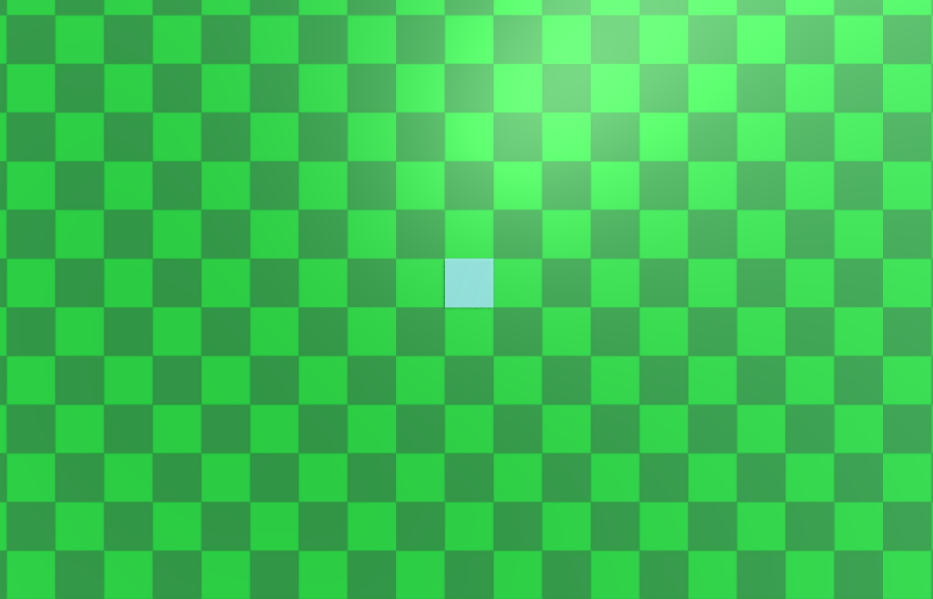
\includegraphics[width = 1\linewidth]{BlankGrid.png}
\end{figure}
This had about the same functionality as curves with the only limitation being at most 8 ways of diversion, which would suffice as intersections in real life only have about 4 directions of travel.
\subsection{One ways Only}
Another decision made mid development, Forcing the user to only create one way roads at first seemed un-intuitive and straying from the goals of the project. However with a little more thought, One way roads made the user's options far greater and kept the program simple. One way roads in essence were the fundamental building block for all roads, as two way roads would just be a two one way roads, roundabouts were round one ways, etc. So even if it took more effort from the user, one way roads compared to other options both simplified the program and also allowed for many possible options for users.
\subsection{Intersections and Right of Ways}
There are 3 types of intersections, lights, stop, and yield, each with their own unique logic. The three chosen were most prominent throughout both literature and the US. There are still few intersections left out with these 3 types but in the scope of the project and targeted user, it did not seem that there would be issues with omitting the other intersection types.

Intersections were implemented through managing collections of cars and giving the right of way to cars whenever their conditions are satisfied. For yield signs that is when there are no cars going in conflicting directions, stops are whenever cars are not in a intersection, while lights are time based. An alternative would be for cars to check for possible conflicts and proceed accordingly, much like real life. Yet the first approach was chosen in order to keep cars from having less logic within them, as most of the time the simulation would have more cars than intersections, meaning more work for the computer.
\subsection{Cars and Movement}
Cars, the most important factor in the simulator were implemented in unique ways due to a variety of reasons. For one, cars gain their path through outside sources, and said outside source must get a path from the A-Star algorithm, however the cars have the capability to path find on their own if prompted. From given paths the car will move very linearly toward their destination, following existing roads. And if ever encountering barriers such as intersections or other cars, the car would slow down accordingly.
\begin{figure}[h]
\caption{A visualization of how Cars path to their next cell in the current path}
%\centering
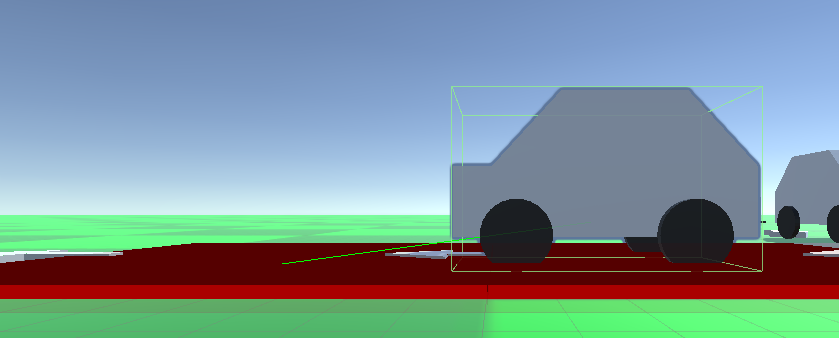
\includegraphics[width=0.45\textwidth]{Nextcell.png}
\end{figure}
\subsection{Braking and Halting}
Braking was implemented similarly to literature previously discussed \cite{roadTrafficModeling}, although with one major caveat. Because cars are moving at a near constant speed except when slowing down the minimum distance required for a car to start braking was allowed to be constant without losing too much realism. But in terms of actual braking it was chosen to have a gradual slow down much like real brakes, as the car gets closer to another vehicle in front of it it slows down more and more. 

Another choice needing to be made was how cars saw their closest cars. There were many options here such as larger triggers that told the car when something was in front of it. Ray cast implementations being another, where a ray would find the closest vehicle. Lastly checking cells list of cars for what car was next from the current car. Due to needing this targeting function to work near perfectly cell checking was chosen as both rays and trigger hit boxes had issues when it came to a car turning, since both had to be positioned on the front of a car or require additional logic not needed with cell checking. 
\begin{figure}[h]
\caption{The current systems of cars finding their target to brake towards, the red floor being their current and next cell and black line symbolizing distance from front of car to back of target}
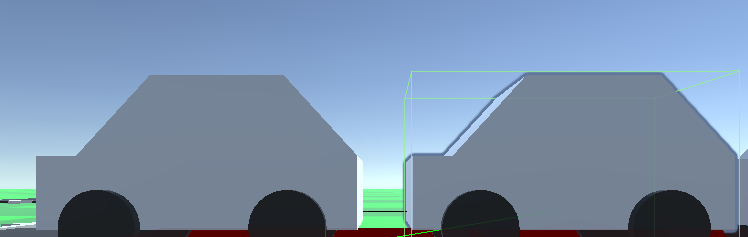
\includegraphics[width=0.45\textwidth]{CellCheckBlackGizmo.png}
\end{figure}
\subsection{Showing Issues in the Network}
Having congestion is natural in a network with too many cars and not enough roads, but showing problems to the user can be difficult in its own ways. It was opted to let the user figure out the issues themselves, due to time constraints, and allowing the user to figure out solution to problems within the network. At present the only real indicator of network congestion is cars turning red after a set amount of time, however it is normally inaccurate when at a light intersection. 
\begin{figure}[h]
\caption{Cars turning red after a constant amount of time stopped}
%\centering
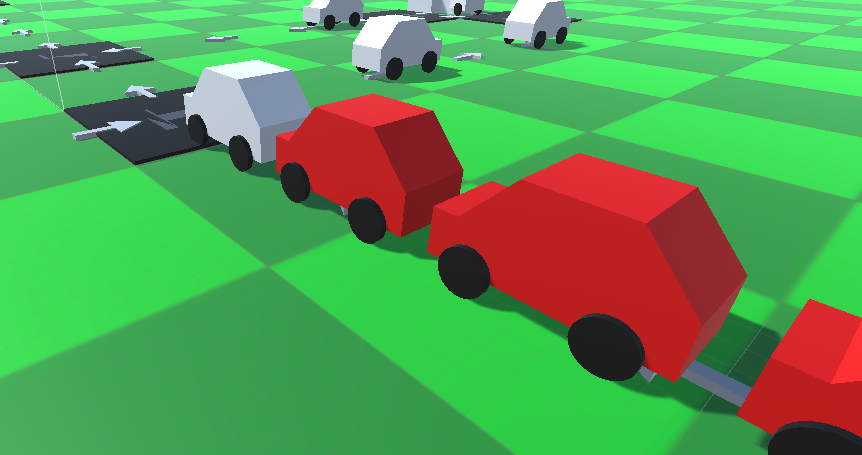
\includegraphics[width=0.45\textwidth]{red.png}
\end{figure}
\subsection{Homes and Headquarters}
Another decision made earlier on was to only use two types of buildings, that being homes and destinations, where a car spawning from home tries to go to destinations, and vice versa. This was done to keep the simulation easier to use, and allow for the project to be finished on time. Other methods of car destinations include adding multiple destinations, random spawning and destinations, and scheduled destinations, but all of these alternatives either took away from the main goals of traffic engineering or were unfeasible with the mechanics already present in the simulation at the time. 
\subsection{The Ins and Outs of Buildings}
Another unique attribute to buildings is there separating inputs and outputs for cars. So the user would have to choose two different adjacent cells in order to have a complete building. This was done to not overwrite a road building principle previously included, where a cell could not have two connections in a single direction, for example a cell's north direction can not have an inward connection and outward connection. So to keep this principle it was chosen to have unique inputs and outputs.
\subsection{The Missing aspects} 
Although the scope of this project is simplicity for education, there were still some omitted functions that might have helped to better emulate traffic or teach. The three second rule \cite{CADMVDrivingManual} was unfortunately not implemented due to time constraints but with it would have lead to more realistic braking. Variable speeds also were not decided to be necessary, because variable speeds would have broken the current braking system. Another system not implemented was lane changing and moving towards right and left lane for turning. This was due to one way roads not having the right logic needed for lane switching, and if it were implemented causing issues to most of the grid. Finally congestion warnings at intersections would also have been possible to implement, but would have to be calculated using functions and variables that could change depending on intersection type and size, as there would need to be a function to get intersection maximum capacity and compare that to current capacity, which is easier said than done.

\section{Evaluation Metrics}
This project was meant to bring people into the sphere of urban planning and traffic engineering, and with that in mind there are certain metrics needed to show completion of the project, along with other pitfall metrics that could have drastically changed my project. 
\subsection{Intersection replication}
\label{replication}
One of the first metrics I created was the ability for a real life intersection to be replicable in the simulation. This metric was done through my own testing with real life intersections, such as streets around where I lived. This test included roundabouts, 4 leg intersections, slanted 4 way intersections, T intersections and even a 4 leg intersection with 2 right slip lanes. Other examples included in the literature were ones such as channelized 4 way roads \cite{GeometricDesign}.
\subsection{Simplicity}
Another metric chosen was how easy it was to understand the simulation. I measured this through the amount of visuals present on the screen at a certain time. I chose this measurement instead of user feedback as there would be potential differing amounts of criticism towards the simulation's front end. User feedback could of caused more focus toward UI and would detract from the actual project, hence why it was avoided.
\subsection{Accuracy of cars}
I wanted to make sure this simulator was a little more accurate than the games previously stated in section \ref{Prior Work} and my only real measurement to this was using the literature I had at hand. As other methods of accuracy such as observing cars in real life can have issues when it comes to human error and larger vehicles. Both of which not present in the simulation.
\subsection{Modularity}
Since one of my goals was to allow the user to explore a sandbox environment I also wanted the user to explore the differing options that each infrastructure had, for example changing traffic light timing on each light, or making it dynamic. To measure this I would see the amount of possibilities a user had when constructing their network, although there is really other alternatives to this way of measuring as modularity is a subjective goal.
\section{Results and Discussion}
Overall I would say that the simulation can do its job quite nicely with being a sandbox for beginners of traffic engineering and urban planning, although it is not without faults as there are some glaring issues in the final product. 
\subsection{Replicating Intersections}
\label{replicatingResults}
Intersection replication was by far the strongest metric as all of the example as each example listen in section \ref{replication} were all possible and only one needed slight modification. With this replication being a success potential users would be able to recreate intersections they personally find interest in and see it in a simulation setting. This replication would most likely not be possible if it were not for the method of one way roads only.
\begin{figure}[h]
\caption{The simulator replication of T-Intersections}
\centering
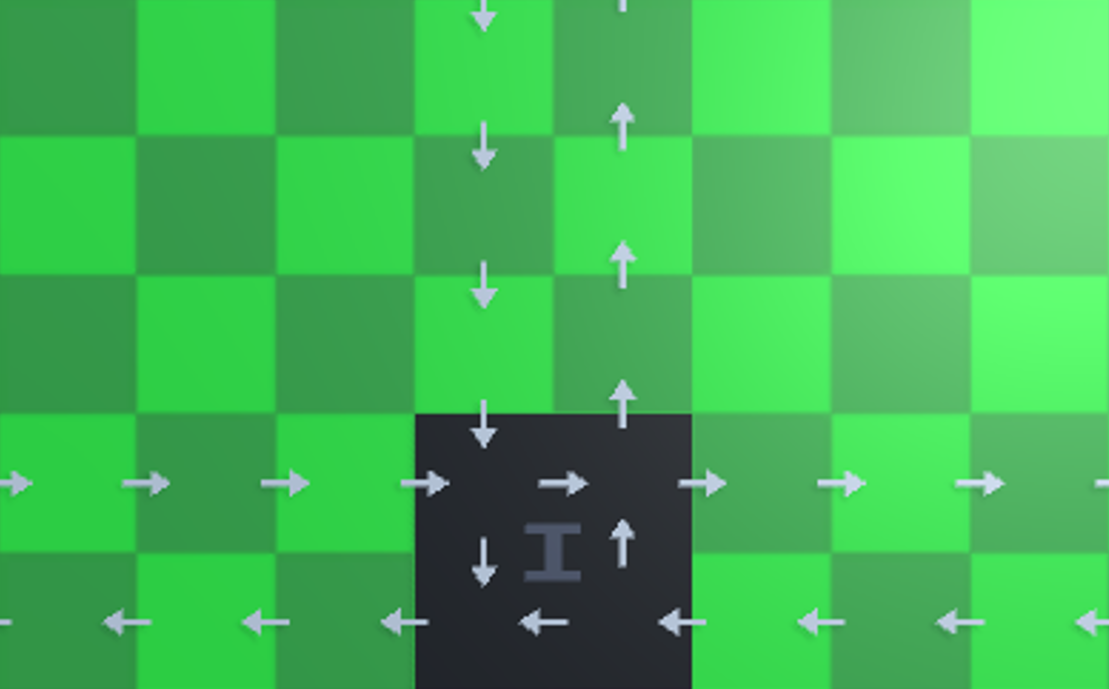
\includegraphics[width=0.4\textwidth]{TZOOMED.png}
\end{figure}
\begin{figure}[h]
\caption{The simulator replication of a 4 way, 2 lane, 2 slip lane intersection}
\centering
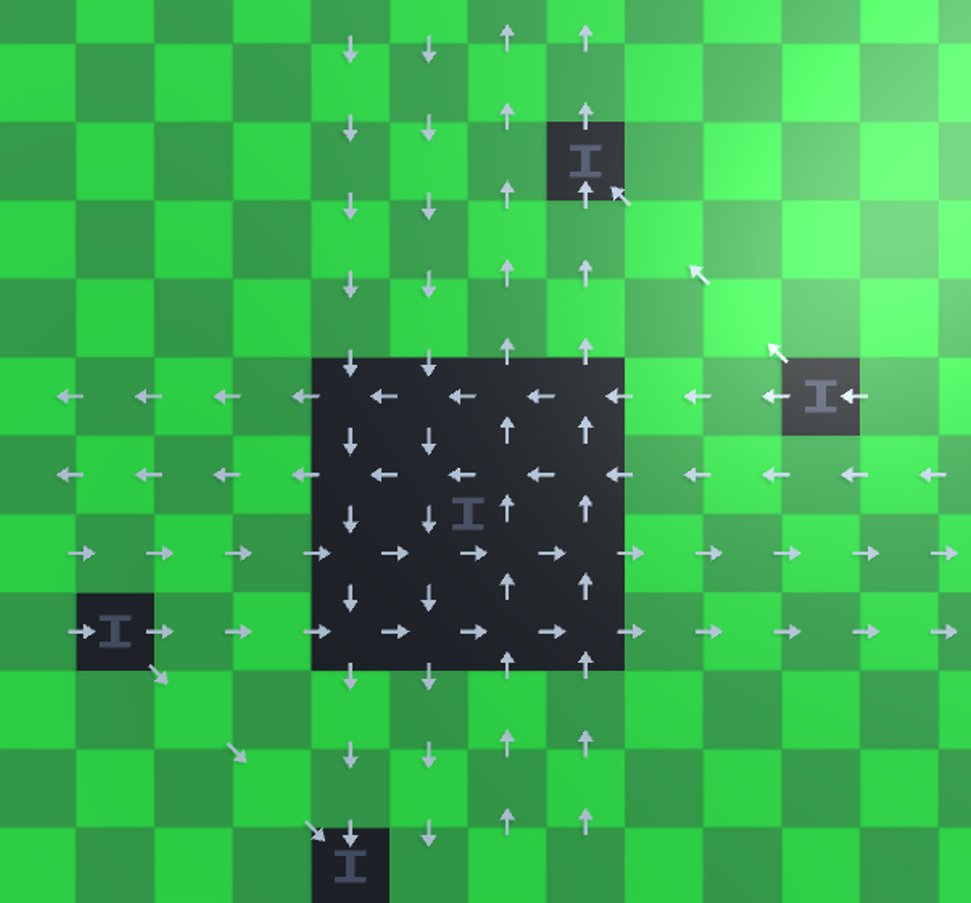
\includegraphics[width=0.45\textwidth]{422ZOOMED.png}
\end{figure}
\subsection{Simplicity}
The simulation itself is also very simplistic, featuring only two different buttons, albeit with one missing due to time constraints. This simplicity would hopefully make the simulator easy to pick up and understand, one of my main goals throughout the project. The Grid based system also makes the simulation easier to see compared to the alternative implementations as if one were to follow arrows they could find where the road ends. The only main issue is the clutter of arrows instead of streets graphics, which was caused due to time constraints forcing me to choose function over graphics. So although there is an issue with visual clutter especially with a larger networks, overall it is serviceable to lower capacity networks, which neighborhood environments should be. Even then, when cars are seen covering up the arrows the simulation looks a lot more understandable. 
\subsection{Car Accuracy}
With regard to car accuracy there are areas of improvement for car behavior. Especially with following distance and braking for cars, as at certain points cars can stop at in a very unrealistic way. This could only be remedied by a whole reworking of the braking system for cars along with the introduction of acceleration to cars and lots of mathematics, but unfortunately due to already having many braking issues and time constraints these were not able to be implemented, causing the less than desirable braking the simulator currently uses. There is also an uncommon bug with housing and braking that stops cars entirely, although it currently, with the braking system, is a tough bug to remove. With this cell checking for the brake target would stay relatively intact as although it has a few issues with targeting, most of the time it was serviceable for finding the right car.
\subsection{Modularity}
Going back to the previous statement about a missing third button in \ref{replicatingResults} that buttons purpose was supposed to allow the user to truly fine tune intersections, from the intersection type to each legs possible sign type, and even measuring the key traffic variables \cite{roadTrafficModeling}, the tuner could also have the capability to tune buildings, however due to time constraints and somewhat complicated design this feature did not make the final product. However using the unity inspector, most of these variables could be changed/read such as changing intersection types, car speed, max cars spawned per building, etc. So although modularity is implemented it is not necessarily accessible through normal means.
\subsection{What comes next}
With all this being said if I were to continue the project there would be many things I would change in order to make a better simulation overall. First of all the fine tuning feature would be implemented first and foremost, as not only is it ready to be implemented, but parts of the UI are present in the simulator, just not shown. Next the overhaul of braking to better represent functions presented within the literature, such as following the three second rule or keeping a following distance speed. Lastly a graphically upgrade to roads would be very helpful to make the simulator look nicer but would require more logic when deciding whether to place a road model or intersection model.
\subsection{What new things could be implemented?}
Keeping with the scope of the project I think there are a few ideas that can be implemented in the future if all previous ideas were implemented. Things such as multiple destinations, dynamic traffic lights, intersection graphics, and moving cameras could all allow even more creativity and less limits within the simulator. Even a little more complexity for the sake of better education, like showing traffic flow throughout intersections could help the user to understand which intersections work well in different situations and densities. 
\section{Ethical Considerations}
Even if this simulation is simple there are still a lot of points of discussion both in the technical terms and more importantly the real life factors omitted from my project. 
\subsection{Human error}
Being a simulator human error would be difficult to implement into the project without either errors such as all traffic stopping or user annoyance as the human error factor would be outside of their control. Although this factor is still very important in the societal context, as traffic engineers must account for human error in order to have functional infrastructure. For example a person may not be looking both ways when turning but in a simulation they know exactly what to do next in order to not crash. Or more subtly a driver taking a few seconds to start moving after the car in front of them already started moving, however in the simulation all cars have an inhuman reaction time of each frame. 
\subsection{Bikes? Busses? Larger Cars?}
Another large group of items omitted are larger or abnormal vehicles, yet another subject that actual traffic engineers absolutely must consider when planning infrastructure, abnormal vehicles are omitted from the project due to the goal of wanting the simulator to be beginner friendly and also because of the possible complexity of these vehicles. For example busses would need multiple destinations, and not only multiple destinations but destinations where they are not destroyed. Larger cars would slow down and speed up differently compared to regular cars, and bikes would have trouble existing on the simulators roads as they would have to take up a whole lane compared to what they usually do in real life where they stick to the right shoulder. These factors missing from the simulation makes this a significant talking point in the societal context. As without them it could potentially lead to dangerous thinking that roads are only meant for cars, however especially outside of North America this is not the case. There are many more vehicle types omitted, taxis, trams, delivery trucks, etc. And while addressed in my literature \cite{StreetElementsToolbox}, this is a problem not easily addressed by a project done in this amount of time but it is certainly a large issue I personally have with my simulator. 
\subsection{America}
With both my literature, lived experiences, and real life examples I can absolutely say that this simulator features American centric ways of traffic engineering. Not only are most of my references from American transit agencies but my real life examples all come from some place in America. There are not dedicated bike lanes like the Netherlands, or pedestrian only walkways that most of Europe and Asia has. This simulator is very much focused on the road and cars only. There are no alternatives in the simulation someone creates, which unfortunately can lead to thinking that the car is the only way to get around. This issue plagues our culture today with self driving cars instead of trains, or wider lanes instead of more options in transportation. And I fear that this simulator may be feeding into that American view of the car. However unfortunate, this project would not be able to address such a large issue in the given time period.
\subsection{One More Lane}
The last societal consideration within this simulator to consider is the fact that simply adding a lane may serve to ease congestion in the simulator. However in real life this has many harmful effects to the people living around the expanded lane. Historical examples include redlining, high cost, more danger to crossing pedestrians, and higher speeds causing catastrophic accidents. All of these factors are important yet overlooked in most cases due to the possible benefit of less congestion. And this simulator only serves to reinforce road widening with no consequences.
\begin{figure}[h]
\caption{Graph from \cite{StreetElementsToolbox} about lane width and vehicle speed}
\centering
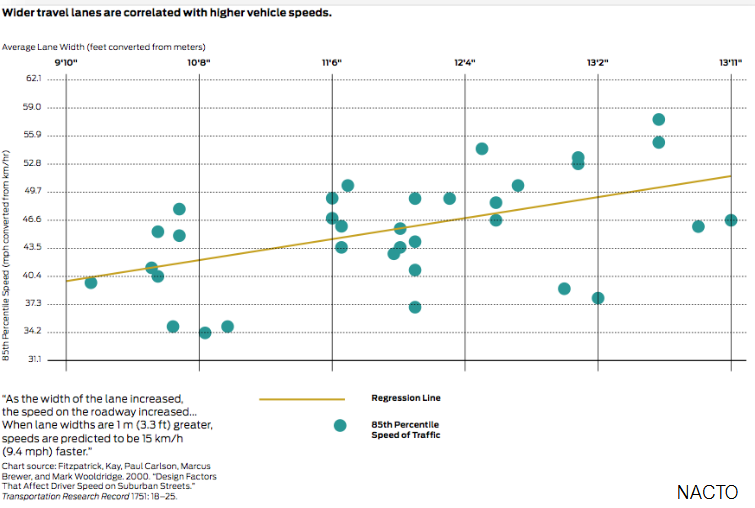
\includegraphics[width=0.5\textwidth]{SpeedChat.png}
\end{figure}
\subsection{Unity}
Moving on to more technical considerations the use of Unity game engine was mainly made due to previous knowledge of it, and although it proved helpful, using real simulating languages and models may have served to help the simulation be more accurate. Although Unity was useful with its unique functions, utilizing another language suited for simulations may have lead to implementation of the omitted functions and features discussed above. 
\section{Project Replication}
Replication of this project is relatively easy, since it is based in unity. Firstly installing Unity Hub and signing in. The project was entirely created in \textbf{Unity Editor Version 2022.3.8f1}, so downloading that version in the installs tab of Unity Hub under official releases, to build the game into an executable file, from the editor go to file and build settings and fine tune the executable instructions and press build. From there unity will create an executable to be able to run. However for testing and future development purposes it is advised to use the unity editor to run the game as it takes much less time to run and can be stopped and modified during run time. Lastly to edit code there are a variety of editors but the main one used was \textit{Visual Studio Code} due to its lightweight design, To set up the IDE of choice, in the unity editor go to edit, preferences then External Tools, from there the external script editor can be chosen through the drop down menu.
\section{Code Architecture Review}
There are few key classes that control most of the code as the simulator was set up with directors guiding other classes into doing tasks. 
\subsection{Cell Head}
The most crucial class of the entire simulator, the Cell Head is in charge of creating, cataloguing, and providing cells. Its serialized inputs are a prefab for cells, a unity grid component, and the group leader. Use Cell Heads public methods in order to create or find cells currently in the simulator. Without this script cells would not be able to be made or kept track of in a centralized area.
\subsubsection{Cells}
Controlled by other scripts the cells are the building block for traffic networks. They have 8 possible directions for either in or out connections and hold what cars are currently on the cell.
\subsection{A Star}
The A star object and script is something that must always be on and always be supplied serially with the Cell Head script, The only method a developer should call from this script is CompleteCoAstar() and constantly at that as this code runs over multiple frames and only returns something that is not null if it found the path or was unable to find the path. Use the variable NoPathIndicator within the script in order to tell whether the returned A Star path is valid or not.
\subsection{Group Leader}
Also known as the intersection leader, supply this with Cell Head, grid, prefabs for errors and intersections and this script will be able to create intersections that can connect to one another, and even merge. The only usable public method is Update Intersection, where given a cell can create an intersection at that cell converting from a road to intersection, however this public method is only usually called by Cell Head when it detects a cell can become an intersection.
\subsubsection{Intersections}
Defaults to lights but can be changed in unity inspector.
\subsection{Selector}
A visualizer for what cell the mouse is currently on, can return the Vector3Int that the mouse is on, through method getGridPos(), which can be interpreted by Cell head to what cell the mouse is currently on.
\subsection{Road Maker}
The Script in charge of making roads of certain directions. Needs the Selector, grid component, a hidden follower that lags behind the selector, Cell Head, and A Star. With all of those components the road maker is able to create roads from mouse drag and drop. Works on its own and calls Cell Head whenever new roads are being made. 
\subsubsection{Roads}
Automatically made through road maker, can only go in one direction.
\subsection{Make Builds}
The building maker, needs grid, 
A Script needing: grid, Selector, Cell Head, A Star, car prefabs, choice prefabs, home prefabs, and destination prefabs. Uses the mouse in order to set up a sequence of choices the user must make to create a car spawner from point A to B, once complete the building will start spawning cars to destination granted there is a path to destination, and vice versa for the destination.
\subsubsection{Cars}
Automatically generated by buildings, has set speed and path when spawned, is destroyed when it reaches its destination.
\subsection{UI and User Mode Select}
The UI and its User Mode Select takes selector, all possible directors, and materials that the selector uses to distinguish its modes, so that whenever the mode is chosen by the UI's buttons that director will activate while others shut off. For example clicking roads actives the road maker and shuts down the building maker. 


\printbibliography
\end{document}
